\section{Introduction}
\label{sec:full_weakintro}
Semantic segmentation is a fundamental computer vision task with applications in numerous domains such as autonomous driving~\sidecite{cordts2016cityscapes,siam2017deep}, scene understanding~\sidecite{sless2019road}, surveillance~\sidecite{tseng2021person} and medical diagnosis~\sidecite{chen2020deep,hesamian2019deep}. As the advent of deep learning has significantly advanced the state-of-the-art, many new application areas have come to light and continue to do so too. This growth has brought and continues to bring exciting domain-specific datasets for segmentation tasks~\sidecite{islam2020semantic,li2020mas3k,Bodenstedt2018,liu2020fsd,WelinderEtal2010}. 

Today, the process of establishing machine learning-based segmentation models for any new application is relatively well understood and standard. Only once an image dataset is gathered and curated, can machine learning models be trained and validated. In contrast, building appropriate datasets is known to be difficult, time-consuming, and yet paramount. Beyond the fact that collecting images can be tedious, a far more challenging task is producing ground-truth segmentation annotations to subsequently train (semi) supervised machine learning models. This is mainly because producing segmentation annotations often remains a manual task. As reported in~\sidecite{Bearman16}, generating segmentation annotations for a single PASCAL image~\sidecite{pascal-voc-2012} takes over 200 seconds on average. This implies over 250 hours of annotation time for a dataset containing a modest 5'000 images. What often further exacerbates the problem for domain-specific datasets is that only the dataset designer, or a small group of individuals, have enough expertise to produce the annotations (\eg, doctors, experts, etc.), making crowd-sourcing ill-suited. 
%\begin{figure*}[t]
%\centering
%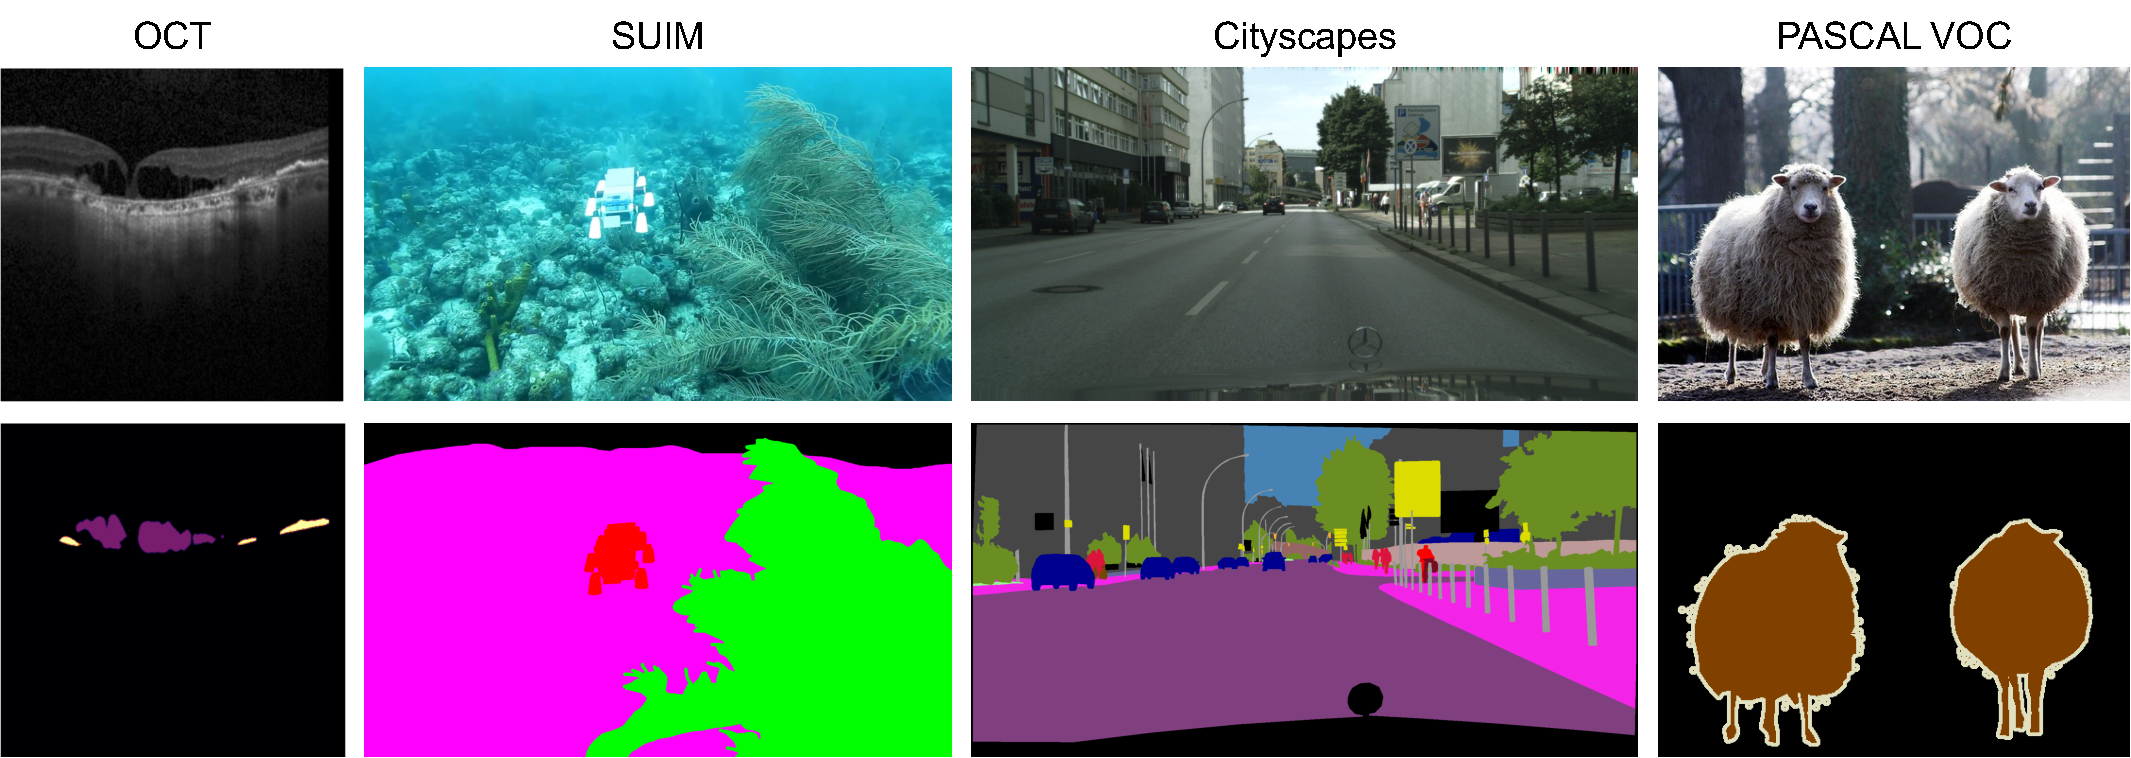
\includegraphics[width=0.99\textwidth]{Figures/datasets.pdf}
%\caption{Illustration of different semantic segmentation applications; OCT: Pathologies of the eye in OCT images, SUIM: Underwater scene segmentation~\sidecite{islam2020semantic}, Cityscape: street level scene segmentation~\sidecite{cordts2016cityscapes}, PASCAL VOC: natural object segmentation.}
%\label{fig:datasets}
%\end{figure*}

\plainwidefig{1}{Figures/datasets.pdf}{Illustration of different semantic segmentation applications; OCT: Pathologies of the eye in OCT images, SUIM: Underwater scene segmentation~\cite{islam2020semantic}, Cityscape: street level scene segmentation~\cite{cordts2016cityscapes}, PASCAL VOC: natural object segmentation.}{fig:fullweak_datasets}

To overcome this challenge, different paradigms have been suggested over the years. Approaches such as Active Learning~\sidecite{Cai21,Casanova2020Reinforced,Konyushkova15} aim to iteratively identify subsets of images to annotate so as to yield highly performing models. Transfer learning has also proved to be an important tool in reducing annotation tasks~\sidecite{Ding2019,heker2020joint,kolesnikov2020big,koleshnikov2021,Liang2020,menegola2017}. For instance, \sidecite{Mensink}~show that training segmentation models from scratch is often inferior to using pre-training models derived from large image classification datasets, even when the target application domain differs from the source domain. Finally, weakly-supervised methods~\sidecite{ahn2018learning,Papandreou15} combine pixel-wise annotations with other weak annotations that are faster to acquire, thereby reducing the annotation burden. In particular, Papandreou~\etal~\sidecite{Papandreou15} showed that combinations of strong and weak annotations (\eg, bounding boxes, keypoints, or image-level tags) delivered competitive results with a reduced annotation effort. In this work, we rely on these observations and focus on the weakly supervised segmentation setting.


In the frame of designing annotation campaigns, weakly-supervised approaches present opportunities for efficiency as well. Instead of completely spending a budget on a few expensive annotations, weakly-supervised methods allow a proportion of the budget to be allocated to inexpensive, or weak, labels. That is, one could spend the entire annotation budget to manually segment available images, but would ultimately lead to relatively few annotations. Conversely, weak annotations such as image-level labels are roughly 100~times cheaper to gather than their segmentation counterparts~\sidecite{Bearman16}. Thus, a greater number of weakly-annotated images could be used to train segmentation models at an equal cost. In fact, under a fixed budget, allocating a proportion of the budget to inexpensive image-level class labels has been shown to yield superior performance compared to entirely allocating a budget to segmentation labels~\sidecite{Bearman16}.

Yet, allocating how an annotation budget should be distributed among strong and weak annotations is challenging, and inappropriate allocations may severely impact the quality of the final segmentation model. For example, spending the entire budget on image-level annotations will clearly hurt the performance of a subsequent segmentation model. Instead, a naive solution would be to segment and classify a fixed proportion of each \sidenote{\eg, 80\% of the budget allocated for segmentation annotations and 20\% for classification.}. Knowing what proportion to use for a given dataset is unclear, however. Beyond this, there is no reason why the same fixed proportion would be appropriate across different datasets or application domains. That is, it would be highly unlikely that the datasets shown in \cref{fig:fullweak_datasets} all require the same proportion of strong and weak annotations to yield optimal segmentation models.

Despite its importance, choosing the best proportion of annotation types remains a largely unexplored research question. Weakly-supervised and transfer-learning methods generally assume that the annotation campaign and the model training are independent and that all annotations are simply available at training time. While active learning methods do alternate between annotation and training, they focus on choosing optimal samples to annotate rather than choosing the right type of annotations. Moreover, most active learning methods ignore constraints imposed by an annotation budget. More notable, however, are the recent works of Mahmood {\it et.~al.}~\sidecite{mahmood2022, mahmood2022optimizing} which aim to determine what weak and strong annotation strategy is necessary to achieve a target performance level. While noteworthy, this objective differs from that here, whereby given a fixed budget, what strategy is best suited for a given new dataset?

To this end, we propose a novel method to find an optimal budget allocation strategy in an online manner\sidedef{online learning}{The data is accessible in a sequential order and is employed to update the model at each step.}. Using a collection of unlabeled images and a maximum budget, our approach selects strong and weak annotations, constrained by a given budget, that maximize the performance of the subsequent trained segmentation model. To do this, our method iteratively alternates between partial budget allocations, label acquisition, and model training. At each step, we use the annotations performed so far to train multiple models to estimate how different proportions of weak and strong annotations affect model performance. A Gaussian Process models these results and maps the number of weak and strong annotations to the expected model improvement. Computing the Pareto optima between expected improvement and costs, we choose a new sub-budget installment and its associated allocation so to yield the maximum expected improvement. We show in our experiments that our approach is beneficial for a broad range of datasets, and illustrate that our dynamic strategy allows for high performances, close to optimal fixed strategies that cannot be determined beforehand.
